\documentclass[11pt,oneside]{article}
\usepackage[T1]{fontenc}
\usepackage[utf8]{inputenc}
%\DeclareUnicodeCharacter{00A0}{ }
\usepackage[adobe-utopia]{mathdesign}

\usepackage{amsmath}
\usepackage[francais]{babel}
\usepackage[dvips]{graphicx}
%\usepackage{here}
\usepackage{framed}
\usepackage[normalem]{ulem}
\usepackage{fancyhdr}
\usepackage{titlesec}
\usepackage{vmargin}

\usepackage{amsmath}
\usepackage{ifthen}
\usepackage{multirow}
\usepackage{multicol} % Portions de texte en colonnes

%\usepackage{xltxtra} % Logo XeLaTeX
%\usepackage{pst-solides3d}
\usepackage{color}
%\usepackage{colortbl}
\usepackage{titletoc} % Pour la mise en forme de la table des matières

%\usepackage[crop=off]{auto-pst-pdf}
%\usepackage{bclogo}


%\usepackage{longtable}
%\usepackage{flafter}%floatants après la référence
%\usepackage{pst-solides3d}
%\usepackage{pstricks}
%\usepackage{minitoc}
%\setcounter{minitocdepth}{4}
%\usepackage{draftcopy}% "Brouillon"
%\usepackage{floatflt}
%\usepackage{psfrag}
%\usepackage{listings} % Permet d'insérer du code de programmation
%\usepackage{lmodern}
%\usepackage[adobe-utopia,uppercase=upright,greeklowercase=upright]{mathdesign}
%\usepackage{minionpro}
%\usepackage{pifont}
%\usepackage{amssymb}
%\usepackage[francais]{varioref}

\setmarginsrb{1.5cm}{1cm}{1cm}{1.5cm}{1cm}{1cm}{1cm}{1cm}

\definecolor{gris25}{gray}{0.75}
\definecolor{bleu}{RGB}{18,33,98}
\definecolor{bleuf}{RGB}{42,94,171}
\definecolor{bleuc}{RGB}{231,239,247}
\definecolor{rougef}{RGB}{185,18,27}
\definecolor{rougec}{RGB}{255,230,231}
\definecolor{vertf}{RGB}{103,126,82}
\definecolor{vertc}{RGB}{220,255,191}
\definecolor{violetf}{RGB}{112,48,160}
\definecolor{violetc}{RGB}{230,224,236}
\definecolor{jaunec}{RGB}{220,255,191}

\usepackage[%
    pdftitle={SLCI -- Introduction aux SLCI -- Applications},
    pdfauthor={Xavier Pessoles},
    colorlinks=true,
    linkcolor=blue,
    citecolor=magenta]{hyperref}



% \makeatletter \let\ps@plain\ps@empty \makeatother
%% DEBUT DU DOCUMENT
%% =================
\sloppy
\hyphenpenalty 10000

\newcommand{\Pointilles}[1][3]{%
\multido{}{#1}{\makebox[\linewidth]{\dotfill}\\[\parskip]
}}


\begin{document}


\newboolean{prof}
\setboolean{prof}{false}
%------------- En tetes et Pieds de Pages ------------
\pagestyle{fancy}
\renewcommand{\headrulewidth}{0pt}

\fancyhead{}
\fancyhead[L]{%
\noindent\noindent\begin{minipage}[c]{2.6cm}
%Lycée Rouvière PTSI

\includegraphics[width=2cm]{png/logo_ptsi.png}%
\end{minipage}
}

\fancyhead[C]{\rule{12cm}{.5pt}}

\fancyhead[R]{%
\begin{minipage}[c]{3cm}
\begin{flushright}
\footnotesize{\textit{\textsf{Sciences Industrielles\\ de l'Ingénieur}}}%
\end{flushright}
\end{minipage}
}

\renewcommand{\footrulewidth}{0.2pt}

\fancyfoot[C]{\footnotesize{\bfseries \thepage}}
\fancyfoot[L]{\footnotesize{2013 -- 2014} \\ X. \textsc{Pessoles}}
\ifthenelse{\boolean{prof}}{%
\fancyfoot[R]{\footnotesize{CI 2 : SLCI -- Applications} \\ \footnotesize{Ch. 1 : Intro aux SLCI -- P}}
}{%
\fancyfoot[R]{\footnotesize{CI 2 : SLCI -- Applications} \\ \footnotesize{Ch. 1 : Intro aux SLCI -- E}}
}


%\begin{center}
%\textit{Centre d'intérêt}
%\end{center}



\begin{center}
 \Large\textsc{CI 2 -- SLCI : Étude du comportement des Systèmes Linéaires Continus Invariants}
\end{center}

\begin{center}
 \large\textsc{Chapitre 1 -- Introduction aux Systèmes Linéaires Continus Invariants} 
\end{center}

\begin{center}
\textsc{Exercices d'application} 
\end{center}

\begin{flushright}
\textit{D'après ressources de Jean-Pierre Pupier} 
\end{flushright}
\vspace{.5cm}

\subsection*{Exercice 1}
\subparagraph*{Question 1}

\textit{Expliquer le fonctionnement des feux tricolores qui règlent la circulation des automobiles dans une intersection.}
\ifthenelse{\boolean{prof}}{
\begin{corrige}

Les feux tricolores peuvent être gérés par une minuterie gérant le changement d'état des feux. 

\end{corrige}
}{}

\subparagraph*{Question 2}
\textit{Pourquoi constituent-ils un système de commande en boucle ouverte ?}
\ifthenelse{\boolean{prof}}{
\begin{corrige}
La présence d'un véhicule ou non sur une voie n'a, dans les feux tricolores les plus simples, aucun impact sur la couleur des feux. 

De plus, rien ne garantit que, que le feu passe réellement au vert au bout d'un certain temps. 

Il n'y a pas de contrôle de la bonne marche du feu (il n'y a pas de rétroaction).
\end{corrige}
}{}


\subparagraph*{Question 3}
\textit{Comment régler la circulation avec plus d'efficacité ? Pour répondre identifier le paramètre important qui n'est pas pris en compte.}
\ifthenelse{\boolean{prof}}{
\begin{corrige}

Une circulation plus fluide peut être obtenue grâce à une détection de présence d'un véhicule. Ainsi la présence d'un véhicule pendant un certain temps sur une certaine voie peut alors provoquer le changement de couleur des feux.

\end{corrige}
}{}

\subparagraph*{Question 4}
\textit{Comment technologiquement mesurer ce paramètre ?}
\ifthenelse{\boolean{prof}}{
\begin{corrige}

\begin{itemize}
\item Détection de la masse du véhicule.
\item Détection du véhicule par boucle d'induction magnétique, le passage du véhicule induisant des courants de Foucault modifiant ainsi l'inductance de la boucle
\end{itemize}

\end{corrige}
}{}

\subsection*{Exercice 2}
On donne un four ainsi qu'un convoyeur sous forme schématique.

Le convoyeur permet de faire transiter une masse de granulats définis par l'utilisateur. Les granulats sont libérés par un actionneur et pesés par un capteur de masse. 

\begin{center}
\begin{tabular}{ccccc}
& 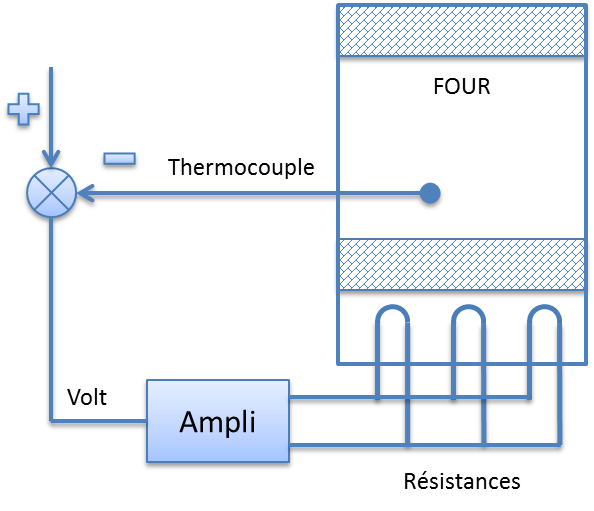
\includegraphics[width=6cm]{png/four} & 
& 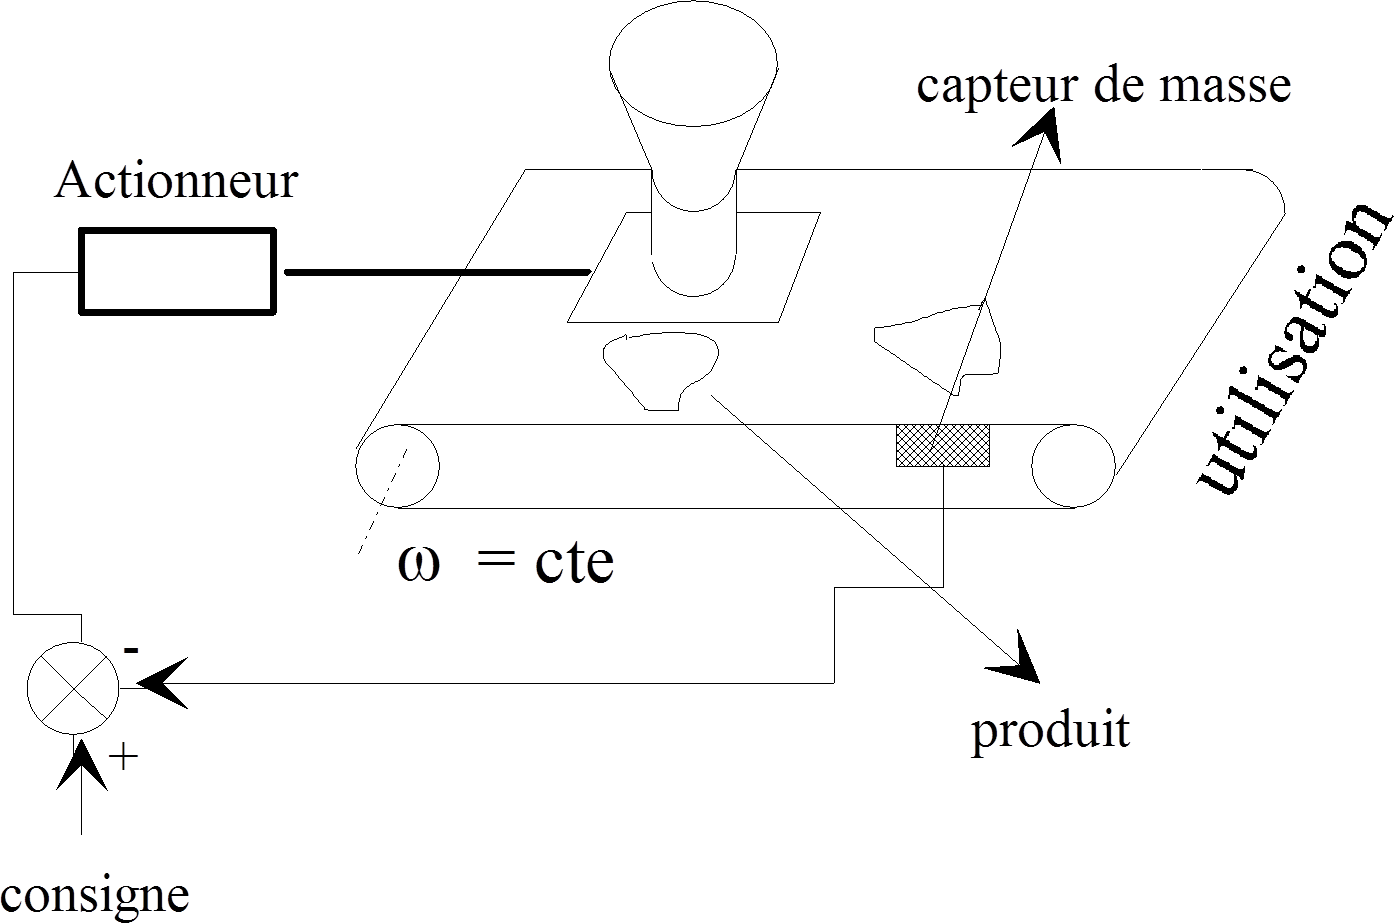
\includegraphics[width=8cm]{png/convoyeur} & \\
\end{tabular}
\end{center}

\subparagraph*{Question 1}
\textit{Pour chacun des deux systèmes, donner une description sous forme de schéma fonctionnel ou schéma-bloc.}
\ifthenelse{\boolean{prof}}{
\begin{corrige}
\textbf{Four}
\begin{center}
 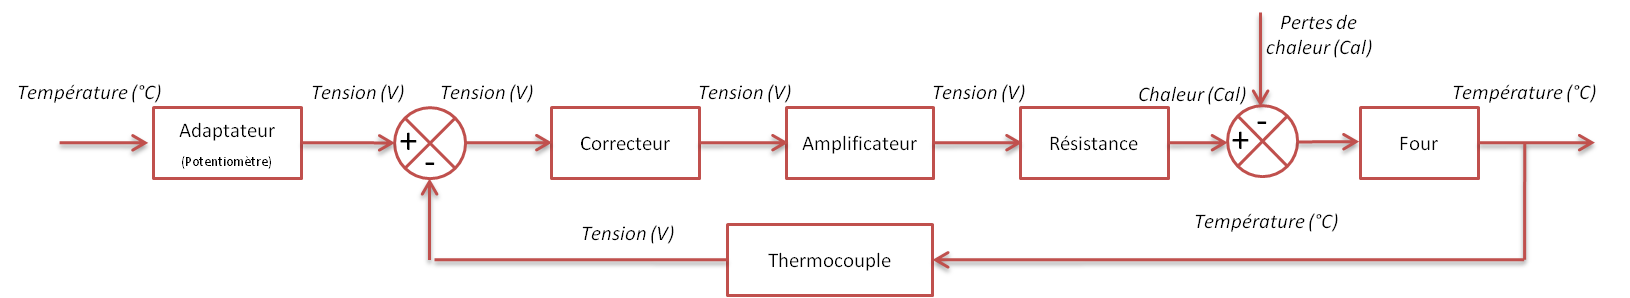
\includegraphics[width=\textwidth]{png/four_cor} 
\end{center}

Le four doit (peut) être considéré comme un bloc à part car la température qui va y régner dépend du volume du four. 

Les thermocouples sont des capteurs utilisés pour mesurer des températures avec une précision de l'ordre de 0,1 \textdegree C. Ils sont constitués de deux conducteurs de matériaux différents reliés soudés à leurs extrémités. Lorsqu'il existe une différence de température existe entre les deux jonctions, un courant apparaît dans le circuit (Effet Seedbeck -- Effet thermoélectrique).  
\end{corrige}
}{}


\ifthenelse{\boolean{prof}}{
\begin{corrige}
\textbf{Tapis roulant}

\begin{center}
 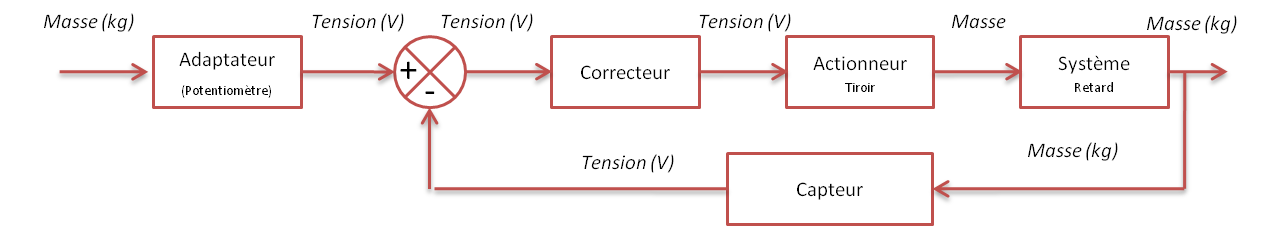
\includegraphics[width=\textwidth]{png/convoyeur_cor} 
\end{center}
\end{corrige}
}{}

%\subparagraph*{Question 2}
%\textit{Même travail que précédemment pour le convoyeur suivant.}

\subsection*{Exercice 3}

La figure ci-après représente un système de régulation de la fréquence de rotation $X$ d'une turbine $T$ grâce à un indicateur de vitesse à boules $I$. 

\begin{center}
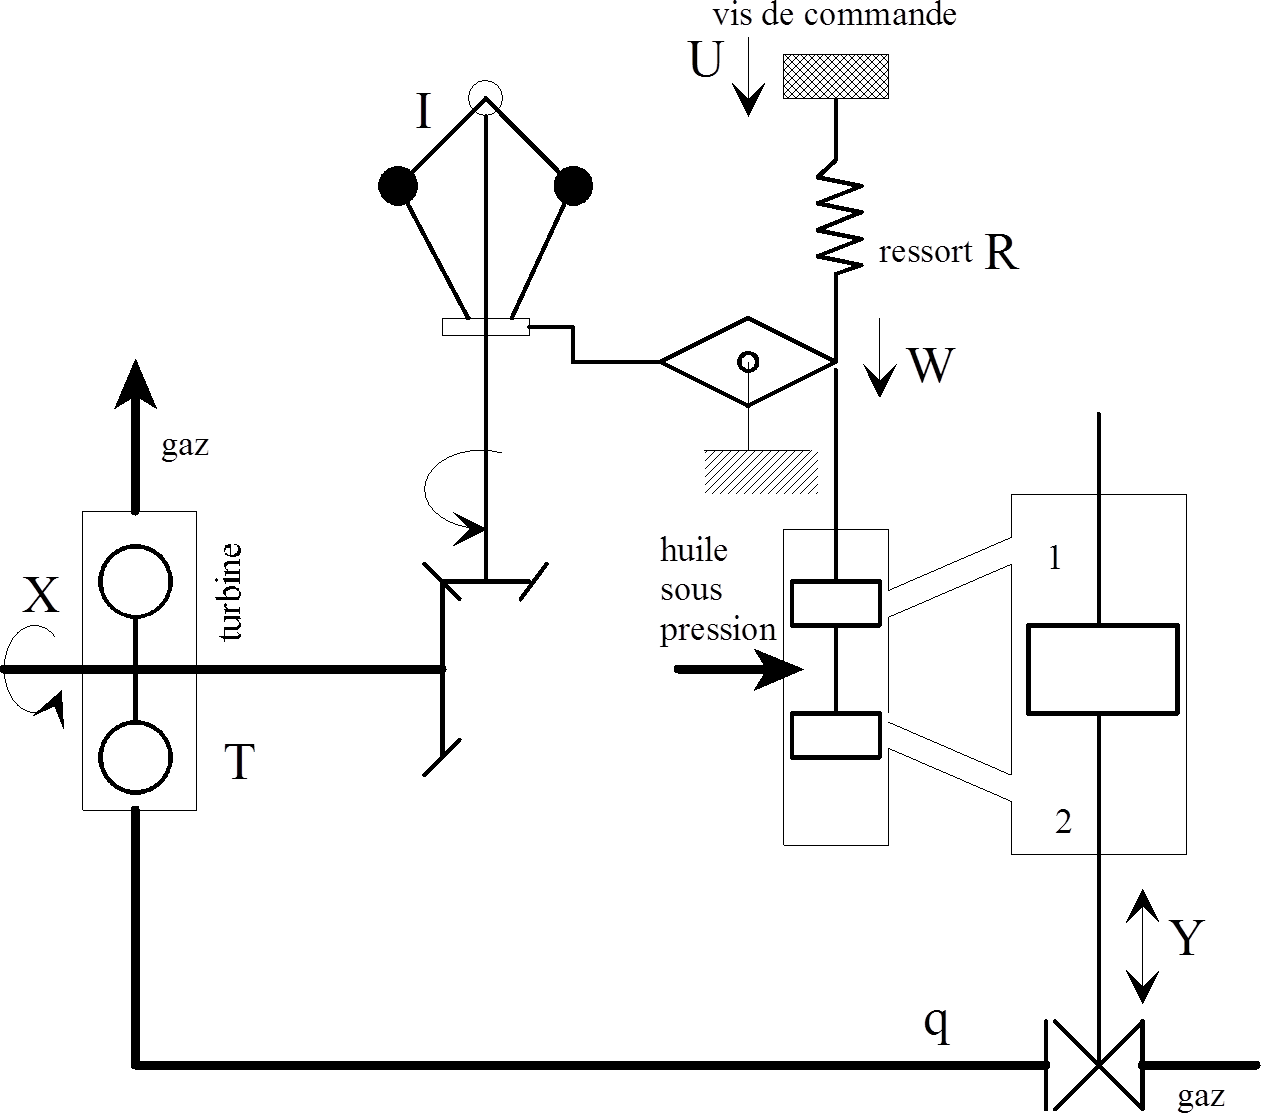
\includegraphics[width=.6\textwidth]{png/regul}
\end{center}

Une turbine permet de transformer de l'énergie cinétique contenue dans des gaz en une énergie mécanique de rotation. 

L'indication de ce capteur de vitesse, centrifuge, est ici renforcée par un amplificateur hydraulique à deux pistons, le déplacement du gros piston commandant l'ouverture de la valve d'admission des gaz dans la turbine. Le déplacement du petit piston résulte de celui de la bague de l'indicateur à boules par le jeu de la force antagoniste d'un ressort R, plus ou moins déplacé d'une quantité U par la vis de commande de l'ensemble du système.

\subparagraph*{Question 1}
\textit{Montrer que ce système est un système asservi.}
\ifthenelse{\boolean{prof}}{
\begin{corrige}

On cherche ici à réguler la fréquence de rotation d'une turbine à gaz grâce à une vis de commande. On se met dans une configuration où la commande est réglée et le ressort est à "l'équilibre".  

Dans cette configuration, de l'huile sous pression est envoyée dans le distributeur hydraulique. L'huile est envoyée dans une des chambres du vérin, fixant ainsi l'ouverture $Y$ de la vanne. 

Pour une ouverture donnée, la vanne délivre un débit $q$ qui génère une fréquence de rotation $X$ de la turbine $T$. La turbine entraîne alors le régulateur centrifuge. Sous les effets de l'inertie, les boules vont provoquer la rotation du levier et donc le déplacement du vérin ce qui produit une fermeture de la vanne. A l'inverse lorsque la fréquence de rotation diminue, sous l'effet de la pesanteur les boules retombent provoquant ainsi la montée du levier et par la suite l'ouverture de la vanne. 

Ce système est équipé d'un dispositif de commande, d'un système permettant de capter la fréquence de rotation de la turbine (via le régulateur) ainsi que d'un levier permettant de comparer la consigne avec une image de la fréquence de rotation. On peut donc parler de système asservi. 


\end{corrige}
}{}

\subparagraph*{Question 2}
\textit{Préciser l'entrée et la sortie.}
\ifthenelse{\boolean{prof}}{
\begin{corrige}
L'entrée est donc la consigne de vitesse donnée par la position $U$ de la vis de commande. La sortie est la fréquence de rotation $X$ de la turbine.

\end{corrige}
}{}

\subparagraph*{Question 3}
\textit{Quels organes constituent le détecteur d'écart, l'amplificateur, l'actionneur, le capteur.}
\ifthenelse{\boolean{prof}}{
\begin{corrige}

Le détecteur d'écart est réalisé par le levier, l'amplificateur par le distributeur, l'actionneur par le vérin, le capteur par le régulateur à boules. 
\end{corrige}
}{}
	 
\subparagraph*{Question 4}
\textit{Réaliser le schéma bloc fonctionnel associé au système.}
\ifthenelse{\boolean{prof}}{
\begin{corrige}

\begin{center}
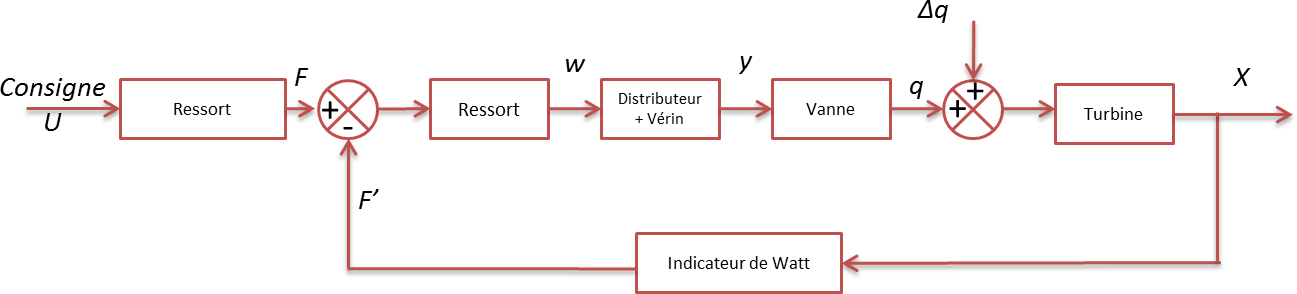
\includegraphics[width=\textwidth]{png/regul_cor}
\end{center}

\end{corrige}
}{}


\end{document}
